\providecommand{\main}{..}
\documentclass[\main/main.tex]{subfiles}

\begin{document}
\graphicspath{{img/}{01_intro/img/}}

\chapter{Introduction}

\section{Problem Statement}
In the modern world, robots play an important role. The interaction between robots and humans help us work faster and more productively. They assist and relieve human operators from dangerous or repetitive tasks. The traditional industrial robots are designed to operate autonomously in isolated spaces. Collaborative robots (or cobots), in contrast, are designed for safely working together or interact with humans in a shared work-space. The safety of cobots may come from the force/torque limitation mechanism. Elastic actuators are good in force/torque control and widely adopted in cobots.

In conventional mechanical design, the joints connecting links, or connecting actuators and loads, are made as stiff as possible. This causes conventional rigid robots to promptly move to expected positions regardless of what external forces/torques act on their joints. This characteristic is adequate for industrial automation because it allows robots for tracking trajectories in static or mapped environments, e.g. pick-and-place applications. In unstructured or dynamic environments, nevertheless, the stiff robot actuators could lead to some issues. First, stiff actuators are not good for force control. The force control is difficult since it develops high forces from small displacement and a little position error can result in a large force error. Furthermore, if the robot is heavy, large forces are required to produce motion, even for small movements. Unfortunately, electrical motors can not generate large forces at high speed. The solution is using gear reductions. Although the gear systems increase torque output, it also generates friction, backlash, and torque ripple. Second, rigid actuators can be damaged by unpredictable collisions or large shock loads. In addition, human operators could be injured by an unexpected collision with a robot arm when collaborating in a shared work-space.

To facilitate the robot to work in dynamic environments or cooperate with humans in a shared work-space, compliant motion and fine torque control are required on each joint. Over the last years, elastic joints have become progressively prominent and are adopted in a variety of new robotic applications. Elastic joints have numerous advantages. Firstly, the elasticity of the elastic elements acts as low-pass filter shock loads, which reduce peak gear forces. In unknown environments, this shock-load tolerance characteristic is very crucial because unexpected collisions can cause damage to the robot actuators. Secondly, friction and mechanical impedance of elastic actuators are low, so that they can achieve high-quality force control. Good force-controlled actuators have several important measures: force bandwidth, mechanical output impedance, dynamic range, power density, and force density. Although the force bandwidth is reduced, elastic actuators have the high force and power density. Actuators with high force density (i.e force-mass ratio) and high power density (i.e power-mass ratio) means that a small actuator can output a lot of energy. Thirdly, potential energy can be stored and released through elastic components, like biological tendons which reduce the work from muscle. Storing energy in the form of potential energy is more energy efficient This could reduce energy consumption, which prolongs battery life in mobile robots and reduces costs.

With many advantages mentioned in the previous paragraph, elastic actuators gradually become popular in robotics, particularly in flexible joint robotic manipulators. However, controlling this type of robot manipulator has some challenges. First of all, the oscillation caused by the elastic component can lead to the instability of the whole system. Diminishing the elastic element oscillation is essential. This will facilitate the position and force/torque control mechanism to function well. Secondly, elastic actuators have low force bandwidth, which means that they slowly respond to the control signal. This is a trade-off between response time and shock load tolerance. Thirdly, controlling the position of an elastic actuator is not an easy task. An elastic actuator can be considered as a cascade of two subsystems: load side subsystem and motor side subsystem. These two parts are connected to each other through an elastic component. This means that the load position cannot be directly controlled but has to be driven through the compression/tension force of the elastic element. As a result, the characteristics of the elastic element, e.g. oscillation and low force bandwidth, directly affect the position control mechanism.

% In general, there are two types of controllers in robotics: centralised and decentralised. This categorisation is based on the ways of arranging the controller. In the centralised robotic controller, one main controller is used to acquire data from the sensors and control the robot. The centralised controller reduces the hardware cost of the robot. However, it also introduces communication latency, increases the complexity of system connection as well as requires a powerful computing unit. In addition, the centralised controller reduces scalability. In the decentralised controller, multiple controllers are used, each one for a specific task. The decentralised controller has numerous benefits compared to the centralised controller. First, a distributed control system reduces the complexity of system connection. As a result, the overall communication latency is reduced because of the reduced number of signals required by the multi-joint controller.  Second, the decentralised control mechanism increases scalability. It is much easier to assemble a module to the system than redesign the whole system. Third, powerful embedded control elements can be utilised in each control unit. This facilitates highly effective dynamic-model-based control algorithms to be utilised in a control unit.

% However, to the best of the author's knowledge, there is not much attention to this topic.
% According to the discussion above, controlling the load position of elastic actuators is a fascinating topic, due to not only its promising potential but also its novelty and challenges. The elastic joint is widely adopted in cobots, especially in flexible joint robotic manipulators. This thesis targets on designing a position controller for elastic actuators. In addition, a 2 DOFs robot arm is also designed to illustrate the effectiveness of the idea.

\section{Thesis Objective}
In this thesis, the objective is to design a controller for a flexible robot manipulator. A centralised and decentralised controller are going to be designed. We are going to compare the effectiveness of both approaches. Besides, the mechanical parts are designed and 3D printed. The mechanical design is built with reference to the previous work of Filippo Sanfilippo et al. As a summary, there are four research objectives arisen in this thesis:\par
1/ Develop a mathematical model of the 2-DOF robot with elastic actuators.\par
2/ Design a 2-loop controller for a single joint, including an MRAC and a fuzzy PI controller.\par
3/ Design a robust nonlinear $H_\infty$ controller.\par
4/ Conduct empirical experiments, then evaluate, compare and conclude the effectiveness of the controllers.

\begin{figure}[H]
    \begin{center}
        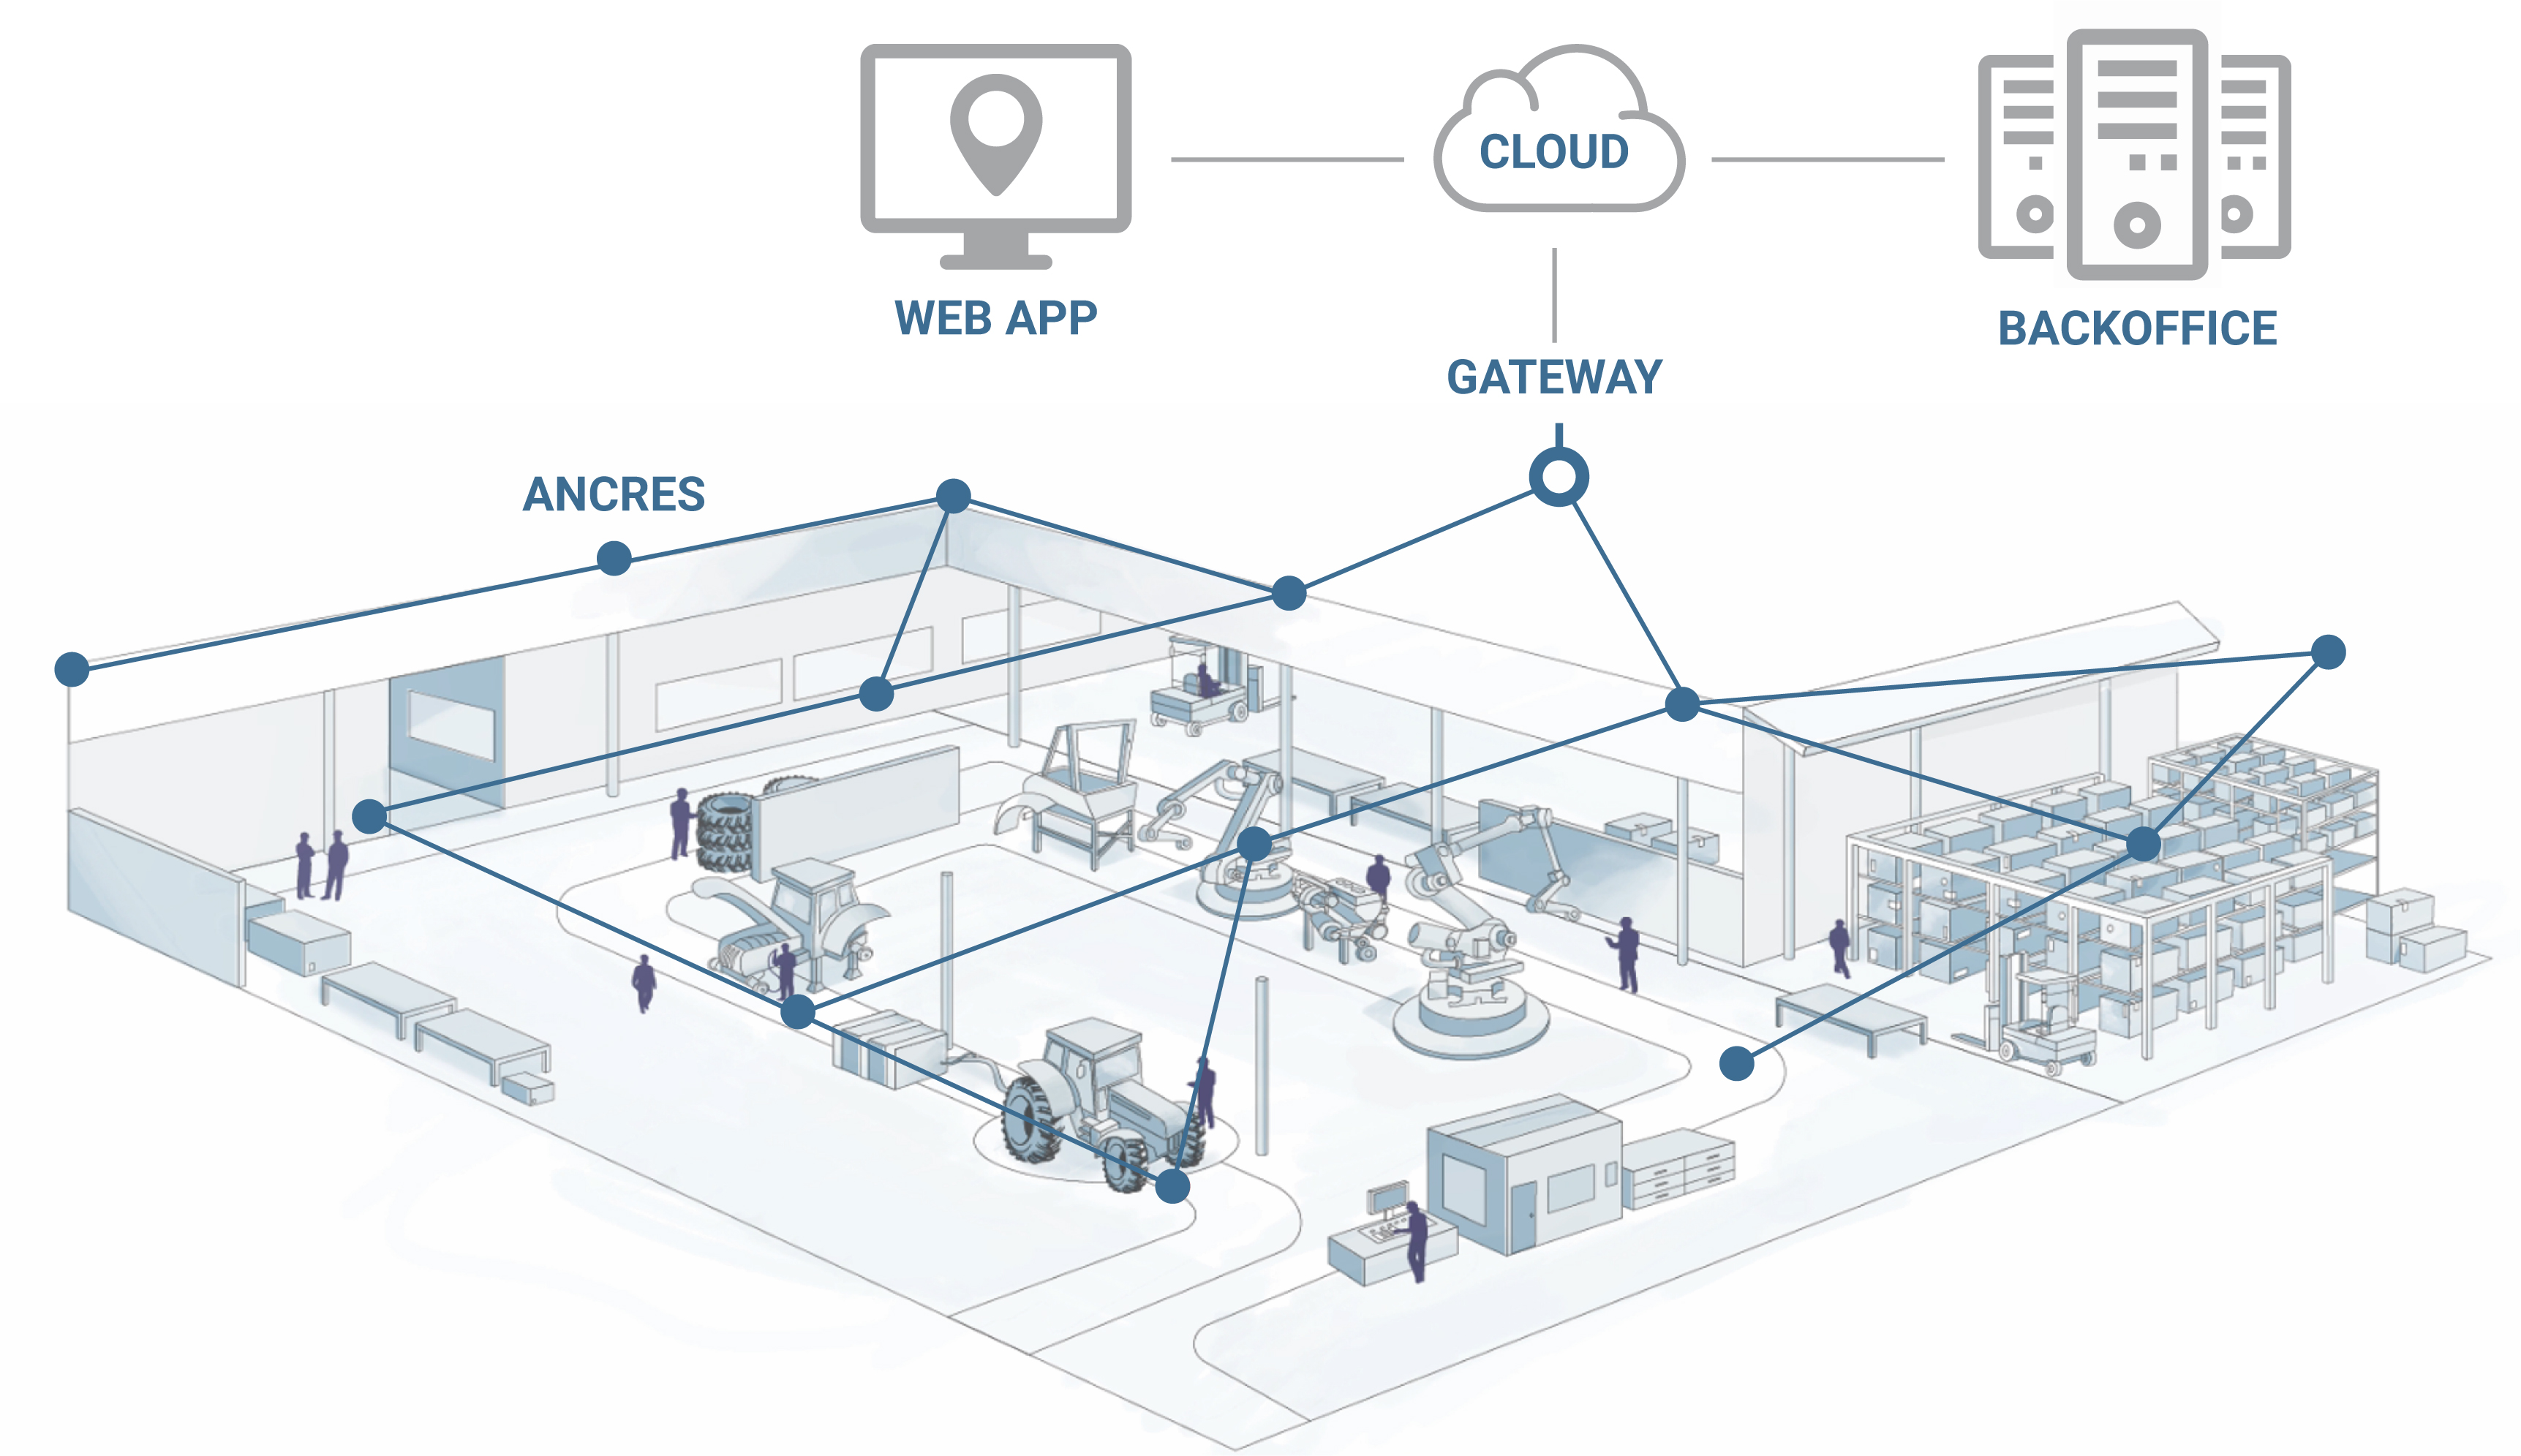
\includegraphics[scale=0.3]{fonctionnement-technologie-mesh-wirepas.jpg}
    \end{center}
    \caption{Indoor location}
    \label{fig:indoor_location}
\end{figure}

\end{document}